\documentclass[journal,twoside,web]{ieeecolor}
\usepackage{generic}
\usepackage{cite}
\usepackage{amsmath,amssymb,amsfonts}
\usepackage{algorithmic}
\usepackage[]{graphicx}
\usepackage{textcomp}
\usepackage{subfigure}
\usepackage{float}
\usepackage{hyperref}
\usepackage{lipsum}
\usepackage{multicol}
\usepackage{caption}
\usepackage[subrefformat=parens]{subcaption} 
%\usepackage[english, czech]{babel}
%\usepackage[useregional]{datetime2}
%\DTMsetdatestyle{czech}
\usepackage[ddmmyyyy]{datetime}
\def\BibTeX{{\rm B\kern-.05em{\sc i\kern-.025em b}\kern-.08em
    T\kern-.1667em\lower.7ex\hbox{E}\kern-.125emX}}
\markboth{ČESKÉ VYSOKÉ UČENÍ TECHNICKÉ V PRAZE, FAKULTA ELEKTROTECHNICKÁ, KATEDRA KYBERNETIKY, \today}
{ČESKÉ VYSOKÉ UČENÍ TECHNICKÉ V PRAZE, FAKULTA ELEKTROTECHNICKÁ, KATEDRA KYBERNETIKY, \today}


\hypersetup{
    colorlinks=true,
    linkcolor=blue,
    filecolor=magenta,      
    urlcolor=cyan,
    pdftitle={Semestrální úloha z předmětu Robotika},
    pdfpagemode=FullScreen,
    }
\begin{document}
\title{Úklid pracovního prostoru}
\author{Aleš Trna, Minh Hoang Tran \\ \begin{center}
    \today
\end{center}
\thanks{}}

\maketitle

\begin{abstract}
    Předmětem této práce je popis řešení závěrečné semestrální úlohy z předmětu Robotika.
\end{abstract}

\begin{IEEEkeywords}
    Robot, manipulátor, počítačové vidění
    \end{IEEEkeywords}

\section{Zadání úlohy}
    V pracovním prostoru robota CRS97 jsou rozmístěny kostky o konstantní velikosti označené
    značkami typu \textit{Aruco}.Robot je umístěn v kleci, která vymezuje jeho pracovní prostor.
    Ke kleci je na konstantním místě připevněna kamera, která zabírá stále stejnou scénu,
    ale ze zadání neznáme její přesnou pozici. Naším úkolem je roztřídit Kostky s \textit{Aruco}
    značkami tak, aby kostky označené stejnými značkami byly uloženy na stejném místě.

\section{Vidění}
\subsection{Kalibrace kamery}
    Abychom mohli detekovat, kde se kostky nacházejí, musíme provést kalibraci kamery. Kalibrací
    kamery zjistíme její distorzi, kterou poté budeme moci kompenzovat, abychom dokázali jednoznačně
    a přesně identifikovat polohu \textit{Aruco} značky vůči kameře.\\
    Princip kalibrace kamery spočívá v nafocení vzorků o známé velikosti a tvaru a porovnávání
    zkreslení výsledného obrázku s realitou. Pro jednoduchost se při této úloze obvykle používá
    Šacovnice o konstantním rozměru čtverce. Pro toto konkrétní řešení byla použita šachovnice
    s \textit{Aruco} značkami na bílých polích o jiném, fixním rozměru díky které byla získána
    přesnější data. Pro co nejpřesnější odhad distorze a parametrů kamery je třeba nafotit co nejvíce
    vzorků z co nejvíce poloh vůči kameře.
    \begin{figure}[h!]
        \centering
          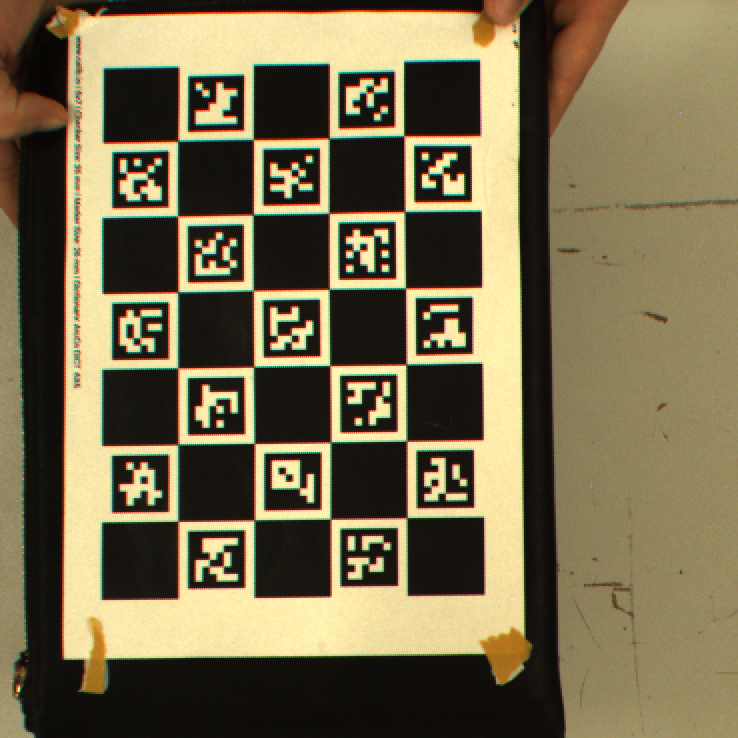
\includegraphics[width=0.45\linewidth]{images/CharucoFlat.png}
          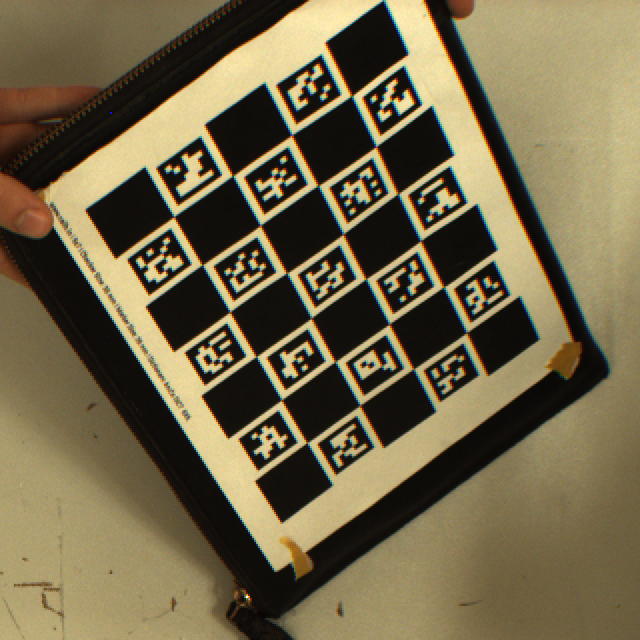
\includegraphics[width=0.45\linewidth]{images/CharucoSkewed.png}
        \caption{Plochá a nakloněná \textit{Charuco} deska}
        \label{fig:CharucoBoard}
    \end{figure}\\
    Na nafocených vzorcích byla detekována \textit{Charuco} deska pomocí funkce \textit{interpolateCornersCharuco}
    z knihovny \textit{cv2}, díky které byla získána Jednoznačná poloha rohů šachovnice a \textit{Aruco} značek.
    Tato data byla použita pro funkci \textit{CalibrateCameraCharuco} ze stejné knihovny.
    Výsledkem byla matice kamery
    \begin{equation}
        \mathbb{C} = \begin{pmatrix}f_x&0&c_x\\0&f_y&c_y\\0&0&1\end{pmatrix}
    \end{equation}
    Kde:
    \begin{itemize}
        \item $f_x$, $f_y$ jsou ohniskové vzdálenosti v konkrétních osách\\
        \item $c_x$, $c_y$ jsou optické středy\\
    \end{itemize}
    Zároveň byly získány distorční koeficienty. Díky kterým můžeme kompenzovat distorzi kamery.

\subsection{Hand to Eye kalibrace}
    Ze zadání úlohy není jasné, kde přesně se kamera vůči robotovi nachází. Je několik způsobů, jak to zjistit.
    Nejjednodušší je změřit polohu kamery vůči pevně zvolenému bodu. Tato metoda je ale pro naše použití
    příliš nepřesná. Dalším způsobem je vytvoření homografické matice, která by nám mapovala scénu kamery
    do roviny. Předmětem této práce je však řešení nerovninného problému, proto tento způsob není vhodný.
    Protože máme již zkalibrovaný obraz z kamery dokážeme díky funkcím knihovny \textit{cv2} zjistit polohu
    objektů. Díky senzorům v robotu známe přesnou polohu chapadla vůči základně robota. V našem konkrétním případě
    není kamera připevněna na chapadle robota, nýbrž na konstrukci v konstantní poloze vůči robotu.
    Řešíme tedy "Hand to Eye" problém. Na jeho řešení můžeme využít opět knihovnu \textit{cv2}, konkrétně
    funkci \hypertarget{cv2Handeye}{\textit{CalibrateRobotWorldHandEye}}. Do chapadla robota vložíme objekt o známých rozměrech,
    u nějž můžeme zjistit jeho polohů vůči kameře. V našem případě využijeme kostku s \textit{Aruco} značkou.
    S robotem budeme jezdit v zorném poli kamery a zaznamenávat scénu pomocí kamery a k ní korespondující
    polohu chapadla vůči základně robota. Poté na fotkách detekujeme polohu \textit{Aruco} značek a data vložíme
    do \hyperlink{cv2Handeye}{zmíněné funkce}. Řešíme tedy rovnici
    \begin{equation}
        \mathbb{A}_i \mathbb{X} = \mathbb{Y}\mathbb{B}_i
    \end{equation}
    Kde:
    \begin{itemize}
        \item $\mathbb{A}_i$ je $i$-tá naměřená transformace chapadla vůči bázi\\
        \item $\mathbb{X}$ je konstantní transformace značky vůči chapadlu robota\\
        \item $\mathbb{B}_i$ je $i$-tá odhadnutá transformace značky vůči kameře\\
        \item $\mathbb{Y}$ je konstantní transformace kamery vůči bázi robota.
    \end{itemize}
    \begin{figure}[h!]
        \centering
          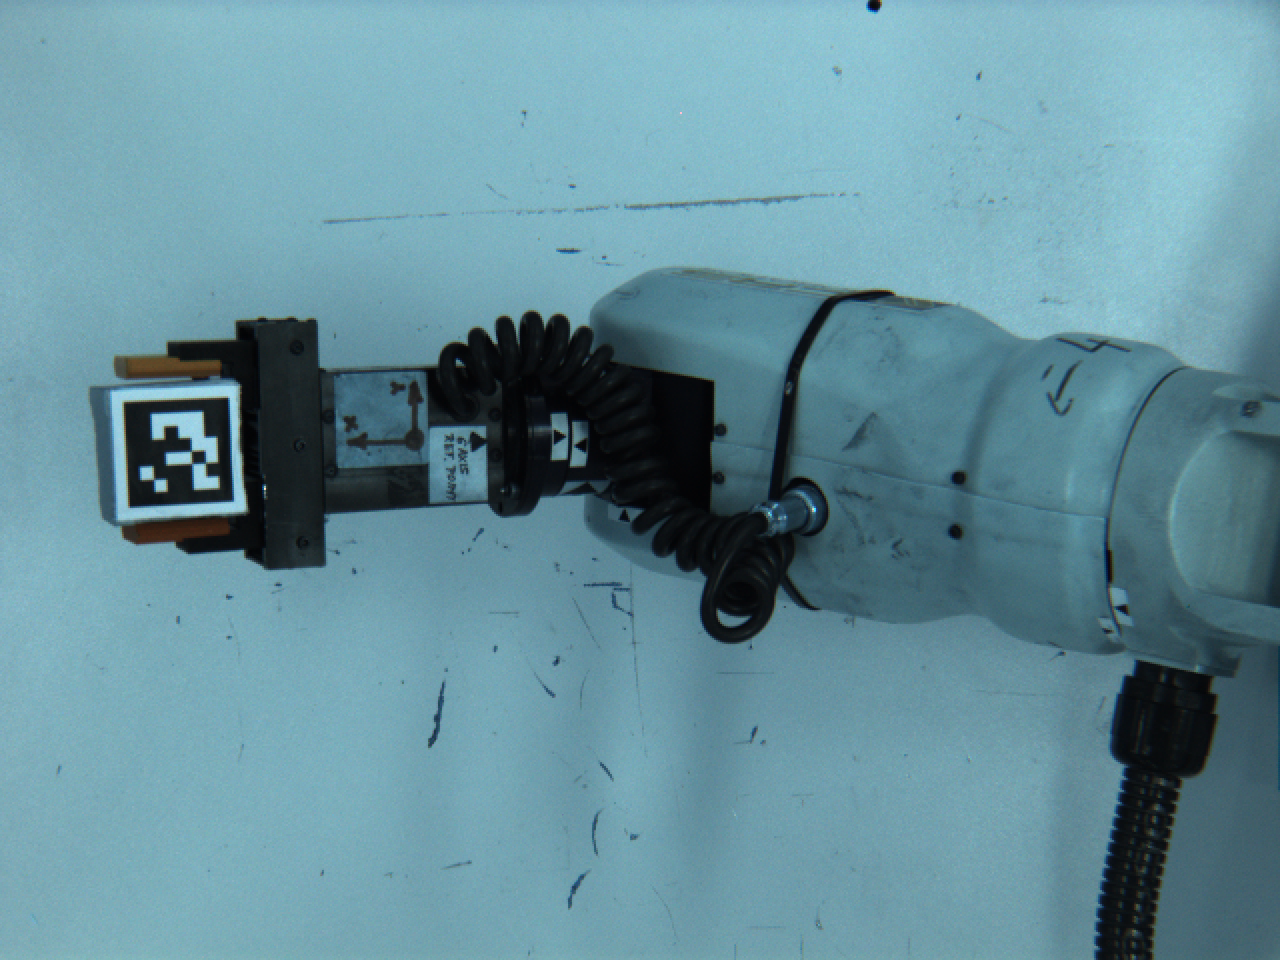
\includegraphics[width=0.8\linewidth]{images/Hand2eye.png}
        \caption{Kostka s \textit{Aruco} značkou uchopená (s konstantní transformací) v chapadle robota}
        \label{fig:ArucoInHand}
    \end{figure}
    Hledáme tedy transformaci $\mathbb{Y}$, pro její výpočet použijeme \hyperlink{cv2Handeye}{výše zmíněnou funkci}.

    \subsection{Korekce transformace}
        Po zjištění polohy kamery vůči základně robota můžeme zjistit polohu kostek vůči robotu. využijeme
        k tomu rovnici
        \begin{equation}
            T_{B\rightarrow K} = T_{B\rightarrow C} \cdot T_{C \rightarrow K}
        \end{equation}
        Kde:
    \begin{itemize}
        \item $T_{B\rightarrow K}$ je transformace kostky vůči bázi robota\\
        \item $T_{B\rightarrow C}$ je transformace kamery vůči bázi robota\\
        \item $T_{C\rightarrow K}$ je transformace kostky vůči kameře\\
        \item Násobení tranformací odpovídá aplikování levé tranformace na transformaci pravou
    \end{itemize}
    Transformaci $T_{C\rightarrow K}$ získáme pomocí \textit{cv2.aruco} funkcí \textit{detectMarkers} a 
    \textit{estimatePoseSingleMarkers}. Jako prvotní test přesnosti kalibrace porovnáme změřenou a spočtenou
    polohu kostek vůči bázi robota. V našem případě jsme zjistili, že robot
    \section{Návrh řešení}
    TODO:\{
    Program je navrhnut jako stavový automat s následujícími stavy:
    \subsection{Inicializační stav}
    \subsection{Třídění podle vrstev}\}
    
\end{document}
